%&pdfLaTeX
% !TEX encoding = UTF-8 Unicode
\documentclass{article}
\usepackage{ifxetex}
\ifxetex
\usepackage{fontspec}
\setmainfont[Mapping=tex-text]{STIXGeneral}
\else
\usepackage[T1]{fontenc}
\usepackage[utf8]{inputenc}
\fi
\usepackage{textcomp}

\usepackage{graphicx}
\usepackage{array}
\usepackage{amssymb}
\usepackage[T2A]{fontenc}
\usepackage[russian]{babel}
\usepackage{fancyhdr}
\renewcommand{\headrulewidth}{0pt}
\renewcommand{\footrulewidth}{0pt}
\usepackage{color}

\definecolor{color17}{rgb}{0.21,0.37,0.57}
\definecolor{color18}{rgb}{0.31,0.51,0.74}

\begin{document}

\vspace{24pt}
\section*{{\large{}{\color{color17} \textbf{Глава 2 Расчет сил осцилляторов\label{HToc453749993}}}}}

\vspace{10pt}
\subsection*{{\large{}{\color{color18} \textbf{2.1 Расчеты ab initio}}}}

\vspace{10pt}
\baselineskip=13pt
{\large{}В работе мы планируем исследовать молекулы 
NaHe, CaF, NeH. Часть параметров, которые нам необходимы 
для использования метода QDT, мы можем узнать, 
произведя компьютерный расчет ab initio основного 
состояния ионов соответствующих молекул. Такими 
параметрами являются вращательные константы, 
дипольные и квадрупольные моменты. Будем использовать 
для этого программы Gaussian 09W и GaussView 5.0.}

\vspace{10pt}
{\large{}Пример кода программы для расчета оптимальной 
конфигурации иона NaHe+.}

\vspace{10pt}
\leftskip=49pt
{\large{}\#p opt MP4/aug-cc-pV5Z}

\vspace{10pt}
{\large{}NaHe}

\vspace{10pt}
{\large{}1 1}

\vspace{10pt}
{\large{}Na             }

\vspace{10pt}
{\large{}He 1 R}

\vspace{10pt}
{\large{}R 2.31}

\vspace{10pt}
\leftskip=0pt
{\large{}Видно, что производится оптимизация межъядерного 
расстояния в ионе NaHe+ методом Мольера-Плиссе 
4-го порядка (MP4) с используемым базисом aug-cc-pV5Z. 
Для молекулы CaF были использованы экспериментальные 
результаты, полученные Jungen в 2001 году.}

\vspace{10pt}
{\large{}Приведем для каждого иона сводную таблицу 
полученных результатов.}

\vspace{10pt}
\begin{tabular}{|>{\raggedright}p{25pt}|>{\raggedright}p{42pt}|>{\raggedright}p{50pt}|>{\raggedright}p{49pt}|>{\raggedright}p{52pt}|>{\raggedright}p{53pt}|}
\hline
М\textbf{етод расчета} & Б\textbf{азис} & B\textbf{ (а.е.)} & Д\textbf{ипольный 
момент, a.u.} & К\textbf{вадрупольный момент, a.u.} & Э\textbf{ффективный 
дипольный момент, a.u.}\tabularnewline
\hline
MP2 & 6-31++g
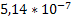
\includegraphics[width=54pt, height=15pt, keepaspectratio=true]{7-fig001.png}
 &  & 0,65 & 0,20 & 0,47\tabularnewline
\hline
MP4 & 6-31++g
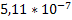
\includegraphics[width=54pt, height=15pt, keepaspectratio=true]{7-fig002.png}
 &  & 0,75 & 0,24 & 0,57\tabularnewline
\hline
 & aug-cc-pVTZ
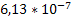
\includegraphics[width=54pt, height=15pt, keepaspectratio=true]{7-fig003.png}
 &  & 0\textit{,60} & 0\textit{,30} & 0,24\tabularnewline
\hline
 & aug-cc-pV5Z
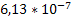
\includegraphics[width=54pt, height=15pt, keepaspectratio=true]{7-fig004.png}
 &  & 0\textit{,60} & 0\textit{,30} & 0,24\tabularnewline
\hline
HF & 6-31++g
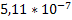
\includegraphics[width=54pt, height=15pt, keepaspectratio=true]{7-fig005.png}
 &  & 0\textit{,75} & 0\textit{,24} & 0,57\tabularnewline
\hline
 & aug-cc-pVTZ
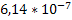
\includegraphics[width=54pt, height=15pt, keepaspectratio=true]{7-fig006.png}
 &  & 0,64 & 0,32 & 0,30\tabularnewline
\hline
CCSD(T) & 6-31++g
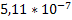
\includegraphics[width=54pt, height=15pt, keepaspectratio=true]{7-fig007.png}
 &  & 0,75 & 0,24 & 0,57\tabularnewline
\hline
 & aug-cc-pVTZ
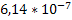
\includegraphics[width=54pt, height=15pt, keepaspectratio=true]{7-fig008.png}
 &  & 0,64 & 0,32 & 0,30\tabularnewline
\hline
\end{tabular}

\vspace{10pt}
\begin{center}
Таблица 4. Ион NaHe+\pagebreak{}
\end{center}

\vspace{23pt}
\baselineskip=13pt
\leftskip=0pt
\begin{tabular}{|>{\raggedright}p{33pt}|>{\raggedright}p{44pt}|>{\raggedright}p{41pt}|>{\raggedright}p{40pt}|>{\raggedright}p{53pt}|>{\raggedright}p{60pt}|}
\hline
М\textbf{етод расчета} & Б\textbf{азис} & B\textbf{ (а.е.)} & Д\textbf{ипольный 
момент, a.u.} & К\textbf{вадрупольный момент, a.u.} & Э\textbf{ффективный 
дипольный момент, a.u.}\tabularnewline
\hline
MP2 & 6-31++g
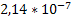
\includegraphics[width=54pt, height=15pt, keepaspectratio=true]{7-fig009.png}
 &  & 5,00 & -1,28 & 5,13\tabularnewline
\hline
MP4 & 6-31++g
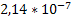
\includegraphics[width=54pt, height=15pt, keepaspectratio=true]{7-fig010.png}
 &  & 5,02 & -1,29 & 5,15\tabularnewline
\hline
 & aug-cc-pVTZ & -- &  &  & \tabularnewline
\hline
 & aug-cc-pV5Z & -- &  &  & \tabularnewline
\hline
HF & 6-31++g
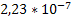
\includegraphics[width=54pt, height=15pt, keepaspectratio=true]{7-fig011.png}
 &  & 4\textit{,91} & -\textit{1,26} & 5,04\tabularnewline
\hline
 & aug-cc-pVTZ & -- &  &  & \tabularnewline
\hline
CCSD(T) & 6-31++g
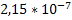
\includegraphics[width=54pt, height=15pt, keepaspectratio=true]{7-fig012.png}
 &  & 5,00 & -1,29 & 5,12\tabularnewline
\hline
 & aug-cc-pVTZ & -- &  &  & \tabularnewline
\hline
\end{tabular}

\vspace{10pt}
\begin{center}
Таблица 5. Ион CaF+

\vspace{10pt}
\begin{tabular}{|>{\raggedright}p{31pt}|>{\raggedright}p{45pt}|>{\raggedright}p{40pt}|>{\raggedright}p{39pt}|>{\raggedright}p{52pt}|>{\raggedright}p{62pt}|}
\hline
М\textbf{етод расчета} & Б\textbf{азис} & B\textbf{ (а.е.)} & Д\textbf{ипольный 
момент, a.u.} & К\textbf{вадрупольный момент, a.u.} & Э\textbf{ффективный 
дипольный момент, a.u.}\tabularnewline
\hline
MP2 & 6-31++g
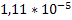
\includegraphics[width=54pt, height=15pt, keepaspectratio=true]{7-fig013.png}
 &  & 1,40 & 0,94 & 1,01\tabularnewline
\hline
MP4 & 6-31++g
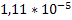
\includegraphics[width=54pt, height=15pt, keepaspectratio=true]{7-fig014.png}
 &  & 1,40 & 0,94 & 1,01\tabularnewline
\hline
 & aug-cc-pVTZ
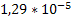
\includegraphics[width=54pt, height=15pt, keepaspectratio=true]{7-fig015.png}
 &  & 1\textit{,17} & 0,89 & 0,70\tabularnewline
\hline
 & aug-cc-pV5Z & --- & -\textit{--} & -\textit{--} & \tabularnewline
\hline
HF & 6-31++g
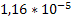
\includegraphics[width=54pt, height=15pt, keepaspectratio=true]{7-fig016.png}
 &  & 1\textit{,35} & 0\textit{,90} & 0,97\tabularnewline
\hline
 & aug-cc-pVTZ
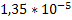
\includegraphics[width=54pt, height=15pt, keepaspectratio=true]{7-fig017.png}
 &  & 1,07 & 0,77 & 0,61\tabularnewline
\hline
CCSD(T) & 6-31++g
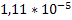
\includegraphics[width=54pt, height=15pt, keepaspectratio=true]{7-fig018.png}
 &  & 1,39 & 0,94 & 1,00\tabularnewline
\hline
 & aug-cc-pVTZ
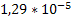
\includegraphics[width=54pt, height=15pt, keepaspectratio=true]{7-fig019.png}
 &  & 1,10 & 0,81 & 0,64\tabularnewline
\hline
\end{tabular}

\vspace{10pt}
Таблица 6. Ион NeH+\label{HToc453749994}
\end{center}

\vspace{10pt}
\subsection*{{\large{}{\color{color18} \textbf{2.2 Определение применимости 
прямого приближения Борна-Оппенгеймера.}}}}

\vspace{10pt}
\baselineskip=13pt
\leftskip=0pt
{\large{}Определим, при каких условиях для исследуемых 
молекул выполняется соотношение }
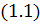
\includegraphics[width=30pt, height=19pt, keepaspectratio=true]{7-fig020.png}
{\large{}, которое позволяет использовать прямое 
приближение Борна-Оппенгеймера.}

\vspace{10pt}
%%\begin{figure}[htbp]
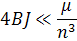
\includegraphics[width=58pt, height=31pt, keepaspectratio=true]{7-fig021.png}
%%\caption{This should be the caption for \texttt{7-fig021.png}.}
%%\end{figure}

\vspace{23pt}
{\large{}Среди серий берем серию с минимальным 
квантовым дефектом. Квантовый дефект усредняем 
по }{\large{}\textit{n.}}{\large{} Для каждой молекулы оцениваем 
}{\large{}\textit{n, }}{\large{}при котором соотношение перестает 
выполняться.}

\vspace{10pt}
\begin{tabular}{|>{\raggedright}p{39pt}|>{\raggedright}p{34pt}|>{\raggedright}p{52pt}|>{\raggedright}p{72pt}|>{\raggedright}p{85pt}|}
\hline
М\textbf{олекула} & \ensuremath{\mu} & С\textbf{ерия} & B\textbf{ 
(а.е.)} & n\tabularnewline
\hline
NaHe & -0,089 & Пd
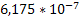
\includegraphics[width=60pt, height=15pt, keepaspectratio=true]{7-fig022.png}
 &  & 33\tabularnewline
\hline
CaF & 0,023 & Дf
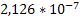
\includegraphics[width=60pt, height=15pt, keepaspectratio=true]{7-fig023.png}
 &  & 30\tabularnewline
\hline
NeH & -0,039 & Уd
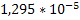
\includegraphics[width=60pt, height=15pt, keepaspectratio=true]{7-fig024.png}
 &  & 9\tabularnewline
\hline
\end{tabular}

\vspace{10pt}
\begin{center}
Таблица 4
\end{center}

\vspace{10pt}
\baselineskip=13pt
\leftskip=0pt
{\large{}Видно, что соотношение перестает выполняться 
при достаточно больших }{\large{}\textit{n}}{\large{}.}

\newpage

\end{document}
